\documentclass[12pt]{article}

\usepackage{graphicx,dcolumn,bm,mathrsfs,subfigure,tikz,pgf,times}
\usetikzlibrary{shapes,arrows}

\begin{document}

\begin{figure}
	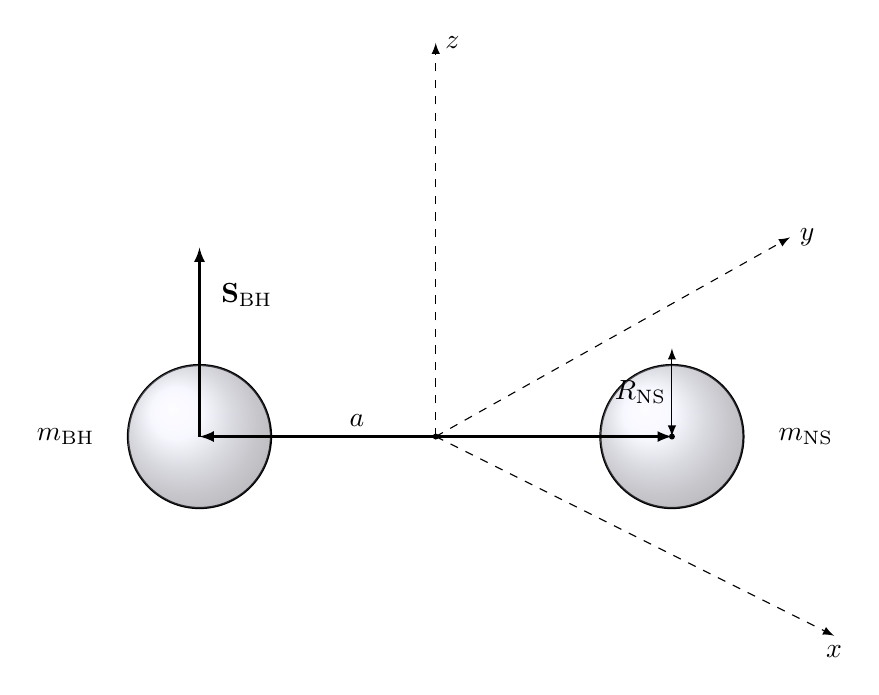
\begin{tikzpicture}[>=latex,scale=2]
		% Draw binary and associated geometry.
		\draw[black,fill=white,thick] (2,0) circle (3ex);
		\shade[ball color=blue!10!white,opacity=0.40] (2,0) circle (3ex);
		\draw[black,fill=white,thick] (-1,0) circle (3ex);
		\shade[ball color=blue!10!white,opacity=0.40] (-1,0) circle (3ex);
		\draw[black,fill=black] (2,0) circle (.1ex);

		% Draw (x,y,z) coordinate frame.
		\draw[dashed,->] (0.5,0) -- (0.5,2.5);
		\draw (0.5,2.5) node[right]{$z$};
		\draw[dashed,->] (0.5,0) -- (2.75,1.2649);
		\draw[dashed,->] (0.5,0) -- (3.0298,-1.2649);
		\draw (3.0298,-1.2649) node[below]{$x$};
		\draw (2.75,1.2649) node[right]{$y$};
		\draw[black,fill=black] (0.5,0) circle(.1ex);

		% Draw binary labels.
		\draw[->,thick] (-1,0) -- (-1,1.2);
		\draw (-0.7,0.9) node{$\mathbf{S}_{\rm BH}$};
		\draw[<->] (2,0) -- (2,0.56);
		\draw (1.8,0.15) node[above]{$R_{\rm NS}$};
		\draw (-1.85,0) node{$m_{\rm BH}$};
        \draw (2.85,0) node{$m_{\rm NS}$};
		\draw (0,0) node[above]{$a$};
		\draw[<->,thick] (-1,0) -- (2,0);
	\end{tikzpicture}
\end{figure}

\end{document}
